\def\QRCODE{TB_IPR_TUT.IMG.binary_morphological_skeletonization_pythonqrcode.png}
\def\QRPAGE{http://www.iptutorials.science/tree/master/TB_IPR/TUT.IMG.binary_morphological_skeletonization/python}
\pcorrectionsection{Python correction}

\begin{python}
from scipy import ndimage
import numpy as np

import imageio
import matplotlib.pyplot as plt
\end{python}

\subsection{Hit or miss transform}

The hit-or-miss transform is illustrated in Fig.\ref{fig:morphological_skeleton:python:elementary}. 
\begin{python}
def hitormiss(X, T):
    """
    hit or miss transform
    X: binary image
    T: structuring element (values -1, 0 and 1)
    
    return: result of hit or miss transform (binary image)
    """
    T1 = (T==1);
    T2 = (T==-1);
    E1 = ndimage.morphology.binary_erosion(X, T1);
    E2 = ndimage.morphology.binary_erosion(np.logical_not(X), T2);
    B = np.minimum(E1, E2);
    return B;

\end{python}

\begin{figure}[htbp]
 \centering\caption{Elementary functions}%
 \subfloat[Hit or miss (intensities are inverted).]{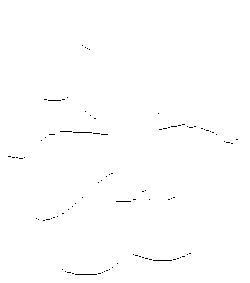
\includegraphics[width=.3\linewidth]{hitormiss.python.png}}\hfill
 \subfloat[Thinning.]{
\includegraphics[width=.3\linewidth]{thinning.python.png}}\hfill
 \subfloat[Thickening.]{
\includegraphics[width=.3\linewidth]{thickening.python.png}}%
 \label{fig:morphological_skeleton:python:elementary}%
\end{figure}


\subsection{Thinning and thickening}
The code is split into 2 elementary operations of thinning and thickening, so that the thinning consists in iterating this operation. The thickening operation is obtained by thinning the complementary set.

\begin{python}
def elementary_thinning(X, T):
    """
    thinning function
    X: binary image
    T: structuring element (values -1, 0 and 1)
    
    return: result of thinning
    """
    B = np.minimum(X, np.logical_not(hitormiss(X, T)));
    return B;
\end{python}
\begin{python}
def elementary_thickening(X, T):
    """
    thickening function
    X: binary image
    T: structuring element (values -1, 0 and 1)
    
    return: result of thickening
    """
    B = not(elementary_thinning(not(X), T));
    return B;
\end{python}

\begin{python}
def thinning(X, TT):
    """
    morphological thinning
    TT is a configuration of 8 pairs of structuring elements
    """
    for T in TT:
        X = elementary_thinning(X, T);

    return X;
\end{python}

\subsection{Skeletons}
The topological skeleton is the iteration of the operation of thinning, for structuring elements defined like:
\begin{python}
TT = [];
TT.append(np.array([[-1,-1,-1],[0,1,0],[1,1,1]]));
TT.append(np.array([[0,-1,-1],[1,1,-1],[0,1,0]]));
TT.append(np.array([[1,0,-1],[1,1,-1],[1,0,-1]]));
TT.append(np.array([[0,1,0],[1,1,-1],[0,-1,-1]]));
TT.append(np.array([[1,1,1],[0,1,0],[-1,-1,-1]]));
TT.append(np.array([[0,1,0],[-1,1,1],[-1,-1,0]]));
TT.append(np.array([[-1,0,1],[-1,1,1],[-1,0,1]]));
TT.append(np.array([[-1,-1,0],[-1,1,1],[0,1,0]]));
\end{python}

\begin{python}
def topological_skeleton(X, TT):
    """
    Topological skeleton: preserves topology
    X: binary image to be transformed
    TT: set of pairs of structuring elements
    return skeleton
    """
    B = np.logical_not(np.copy(X));
    while not(np.all(X == B)):
        B = X;
        X = thinning(X, TT);
    return B;
\end{python}


The topological skeleton is the iteration of the thinning with structuring elements in all 8 directions. It has the property of preserving the topology of the discrete structures, contrary to the morphological skeleton (see Fig.\ref{fig:morphological_skeleton:python:skeletons}).
The morphological skeleton does not preserve the connexity of the branches, but it can be used to reconstruct the original image. Pay attention to the construction of structuring elements, which should be homothetic ($B_r=\underbrace {B_1\oplus \cdots \oplus B_1}_{{r{\mbox{ times}}}}$).
\begin{python}
def morphological_skeleton(X):
    """ 
    morphological skeleton 
    X: binary image
    using disk structuring elements
    
    in order to perform the reconstruction from the skeleton, one has to store 
    the value of S for each size of structuring element
    
    return: S, morphological skeleton, grayscale image
    """
    strel_size = -1;
    pred = True;
    S = np.zeros(X.shape);
    se = ndimage.generate_binary_structure(2, 1);
    E = np.copy(X);
    while pred:
        strel_size+=1;
        E = ndimage.morphology.binary_erosion(X, se);
        if np.all(E==0):
            pred = False;
        D = ndimage.morphology.binary_dilation(E, se);
        S = np.maximum(S, (strel_size+1)*np.minimum(X, np.logical_not(D)));
        X = E;
    return S;
\end{python}

\begin{python}
def reconstruction_skeleton(S):
    """
    Reconstruction of the original image from the morphological skeleton
    S: Skeleton, as constructed by morphological_skeleton
    
    return: original image I
    """
    X = np.zeros(S.shape).astype("bool");
    n = np.max(S);
    se = ndimage.generate_binary_structure(2, 1);
    
    for strel_size in range(int(n)):
        Sn = S == strel_size+1;
        
        # this is for preserving homothetic structuring elements
        for k in range(strel_size):
            Sn = ndimage.morphology.binary_dilation(Sn, se);
        
        X = np.maximum(X, Sn);
    return X;
\end{python}
 
\begin{figure}[htbp]
 \centering\caption{Skeletons. The topology is not preserved in the morphological skeleton, but it can be used to reconstruct the original image. The intensities are inverted in order to facilitate the display.}%
 \subfloat[Topological skeleton.]{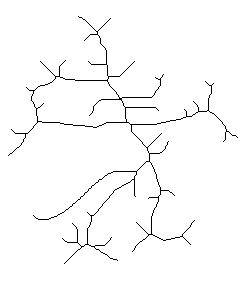
\includegraphics[width=5cm]{topological_skeleton.python.png}\label{fig:morphological_skeleton:python:skeletons:topological_skeleton}}\hspace*{1cm}
 \subfloat[Morphological skeleton.]{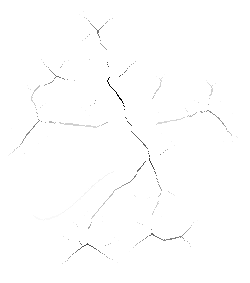
\includegraphics[width=5cm]{morphological_skeleton.python.png}\label{fig:morphological_skeleton:python:skeletons:morphological_skeleton}}%
 \label{fig:morphological_skeleton:python:skeletons}%
\end{figure}

